\documentclass{classrep}
\usepackage[utf8]{inputenc}
\usepackage{amsmath}
\usepackage{graphicx}
\usepackage{url}
\usepackage{hyperref}
\usepackage[T1]{fontenc}
\usepackage[polish]{babel}
\usepackage[utf8]{inputenc}
\usepackage{lmodern}
\usepackage{color}
\usepackage{listings}
\selectlanguage{polish}
\graphicspath{ {./rys/} }


\studycycle{Informatyka, studia dzienne, inż I st.}
\coursesemester{VI}

\coursename{Sztuczna inteligencja i systemy ekspertowe}
\courseyear{2019/2020}

\courseteacher{dr inż. Krzysztof Lichy}
\coursegroup{wtorek, 10:30}

\author{
  \studentinfo{Radosław Grela}{216769} \and
  \studentinfo{Jakub Wąchała}{216914}
}

\title{Zadanie 2: Sieć neuronowa}

\begin{document}
\maketitle
\section{Cel}
Zadanie 2 polega na zaprojektowaniu i zaimplementowaniu sieci neuronowej, która pozwoli na korygowanie błędów uzyskanych z systemu pomiarowego. Do nauki sieci neuronowej należało wykorzystać dane pomiarowe z 12 przejazdów testowych zawarte w plikach z rozszerzeniem .xlsx. Następnie, za pomocą pliku testowego porównaliśmy uzyskane wyniki. \cite{zadanie}
\section{Wprowadzenie}
Wielowarstwowy perceptron to (MLP - MultiLayer Perceptron) to jeden z najpopularniejszych typów sieci neuronowej. Składa się zazwyczaj z jednej warstwy wejściowej i wyjściowej oraz kilku warstw ukrytych. Ilości neuronów w poszczególnych warstwach musi zostać ustalona przez twórcę. \cite{mlp}

Neuron w rozumowaniu matematycznym / informatycznym to pewnego rodzaju sumator, który oblicza sumę ważoną, a następnie podstawia ją do funkcji aktywacji. Wynikiem tej operacji jest wyjście neuronu. \cite{neuron}

Nauka takiej sieci neuronowej polega na nieustannym zmienianiu wag neuronu w taki sposób, aby błąd był jak najmniejszy. Realizuje się to za pomocą wstecznej propagacji błędów. 
\begin{figure}[h!]
	\centering
	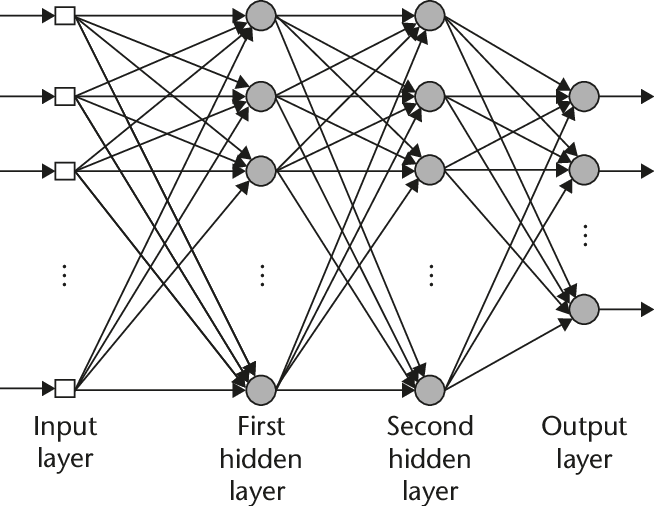
\includegraphics[width=0.8\textwidth]{mlpr.png}
	\caption{Przykładowy schemat sieci neuronowej MLP. \cite{mlpr}}
\end{figure}
\newpage
\subsection{Opis architektury sieci neuronowej}
Nasza sieć neuronowa wykorzystana do rozwiązania problemu korygowania błędów systemu pomiarowego posiada następujące właściwości:
\begin{enumerate}
	\item Liczba warstw sieci neuronowej: 2
	\item Liczebność neuronów w poszczególnych warstwach: 3, 2
	\item Funkcje aktywacji zastosowanych w poszczególnych warstwach: ,,Relu'', czyli  \textsl{rectified linear unit}, f(x) = max(0, x)
\end{enumerate}

\subsubsection{Liczba próbek z poprzednich chwil czasowych} 
Aby przeprowadzić proces nauki sieci neuronowej wykorzystywane są wszystkie próbki z 12 plików testowych. Jest to liczba 18480 próbek $(12 * 1540)$

\subsubsection{Wagi poszczególnych neuronów w warstwach} 
Poniżej zamieszczono wagi poszczególnych neuronów we wszystkich warstwach. Jedna linia w nawiasach kwadratowych reprezentuje jeden neuron.
\begin{verbatim}
1. warstwa ukryta
[ 0.85605396 -0.8344208 ]
[ 0.41779025  0.40123822]
[-0.2743517   0.65437693]
2. warstwa wyjściowa
[ 0.56129234  1.19838389 -0.00534168]
[ 0.02747517  0.7267963   1.04682753]
\end{verbatim}
\subsection{Opis algorytmu uczenia sieci neuronowej}
Sieć neuronowa została nauczona za pomocą algorytmu ,,Adam''. Jest to stochastyczny optymalizator gradientowy. Wybraliśmy go, ponieważ dobrze nadaje się do badania dużych zbiorów danych (co najmniej kilka tysięcy danych treningowych). \cite{doc} 

Algorytm ,,Adam'' został zaproponowany przez Jimmy Lei Ba oraz Diederik P. Kingma. Jest algorytmem optymalizującym pewną zadaną funkcję kosztu opierającym się na \textsl{stochastic gradient descent}. Główna różnica między zwykłym stochastic gradient descent a Adamem polega na liczeniu przesunięcia wartości nie tylko na podstawie aktualnego gradientu, ale również poprzednich.
Wpływ gradientu na kolejne przesunięcia spada jednak wykładniczo. Pamiętanie poprzednich gradientów nie tylko pozwala na szybszą naukę, ale nawet osiąganie lepszych wyników przy tej samej architekturze. \cite{adampl} 

Algorytm przebiega w następujący sposób \cite{adamdzialanie}:
\begin{enumerate}
	\item Obliczenie wykładniczo średniej ważonej przeszłych gradientów i zapisanie ich do zmiennych VdW i Vdb (przed korektą odchylenia) oraz VdWcorrected i Vdbcorrected (z korekcją odchylenia).
	\item Obliczenie wykładniczo ważoną średnią kwadratów poprzednich gradientów i zapisanie ich w zmiennych SdW i Sdb (przed korektą odchylenia) oraz SdWcorrected i Sdbcorrected (z korekcją odchylenia).
	\item Aktualizacja parametrów w kierunku opartym na łączeniu informacji z „1” i „2”.
\end{enumerate}

\section{Opis implementacji i kod źródłowy} 
Napisany przez nas program jest aplikacją w języku Python. Do zaimplementowania sieci neuronowej skorzystaliśmy z biblioteki sklearn. \cite{doc} Projekt składa się z dwóch plików: FileReader.py, zawierający klasę odpowiedzialną za wczytanie plików z danymi treningowymi oraz testowymi. Drugi plik, Main.py, odpowiada za sterowanie programem oraz siecią neuronową.

\subsection{FileReader.py}

\lstinputlisting[language=Python]{../Zadanie2/FileReader.py}

\subsection{Main.py}

\lstinputlisting[language=Python]{../Zadanie2/Main.py}


\section{Materiały i metody}
Do przeprowadzenia nauki sieci neuronowej użyliśmy 12 plików z danymi pomiarowymi przejazdu robota. Następnie, do sprawdzenia wyników nauczenia się sieci neuronowej wykorzystaliśmy plik z danymi testowymi. \cite{pliki}

\subsection{Średnie wyniki}
W tej sekcji przedstawione zostanie 10 uruchomień programu wraz z uzyskanym błędem średniokwadratowym. Wyniki zostaną przedstawione w formie tabeli wraz ze średnią z tych wyników.

\subsection{Porównanie dystrybuant błędu pomiaru dla danych ze zbioru testowego oraz dla danych uzyskanych w wyniku filtracji przy użyciu sieci neuronowej}
W tym eksperymencie zostanie porównana dystrybuanta błędu dla danych ze zbioru testowego oraz dla danych uzyskanych w wyniku filtracji. Stan, jaki zostanie przedstawiony to stan, dla którego w tabeli średnich wyników błąd średniokwadratowy był najmniejszy.


\section{Wyniki}

\subsection{Średnie wyniki}

\begin{center}
	\begin{tabular}{c c} 
		\hline
		l.p. & błąd średniokwadratowy \\ [0.5ex] 
		\hline\hline
		1 & 177.15926881905335  \\ 
		2 & 202.3597557362831 \\
		3 & 177.83635802867894 \\
		4 & 176.54373960197958 \\
		5 & 193.51257888666163  \\
		6 & 152.11542952911833  \\
		7 & 186.3669723390483  \\
		8 & 191.7291476240959  \\
		9 & 202.73906790249782  \\
		10 & 184.05795340024943  \\
		\hline
		\hline
		 &średnia: 184,44  \\		
		\hline
	\end{tabular}
\end{center}

\newpage
\subsection{Porównanie dystrybuant błędu pomiaru dla danych ze zbioru testowego oraz dla danych uzyskanych w wyniku filtracji przy użyciu sieci neuronowej}

\begin{figure}[h!]
	\centering
	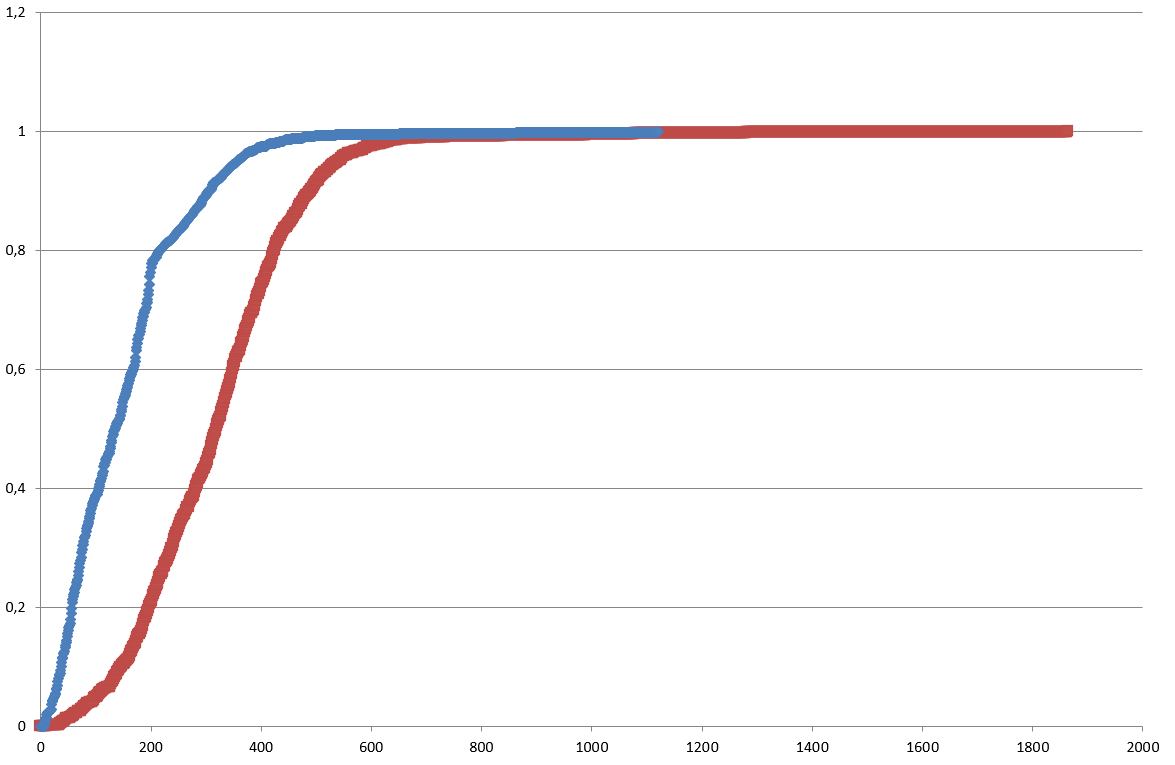
\includegraphics[width=1\textwidth]{dystrybuanta.png}
	\caption{Porównanie dystrybuant błędu pomiaru.}
	\label{dystrybuanta}
\end{figure}



\section{Dyskusja i wnioski} % 6. Dyskusja  %
Jak można zauważyć na rysunku \ref{dystrybuanta}, wyniki filtracji dały lepsze wyniki dystrybuanty błędu. 

\begin{thebibliography}{0}
  	\bibitem{zadanie} \textsl{https://ftims.edu.p.lodz.pl/mod/page/view.php?id=73137} [dostęp 08.05.2020]
	\bibitem{mlp} \textsl{https://pl.wikipedia.org/wiki/Perceptron\_wielowarstwowy} [dostęp 08.05.2020]
	\bibitem{mlpr} \textsl{https://www.researchgate.net/publication/244858164/figure/fig2/AS:
		670028080902154@1536758551608/Structural-graph-of-multilayer-
		perceptron-MLP-neural-network-model.png} [dostęp 08.05.2020]
	\bibitem{neuron} \textsl{https://pl.wikipedia.org/wiki/Neuron\_McCullocha-Pittsa} [dostęp 08.05.2020]
	\bibitem{adam} \textsl{https://arxiv.org/pdf/1412.6980.pdf} [dostęp 08.05.2020]
	\bibitem{doc} \textsl{https://scikit-learn.org/stable/modules/generated/sklearn.neural\_network.
		MLPRegressor.html} [dostęp 08.05.2020]
	\bibitem{adampl} \textsl{https://piotrmicek.staff.tcs.uj.edu.pl/machine-learning/docs/szymon-
		stankiewicz-lincencjat.pdf} [dostęp 08.05.2020]
	\bibitem{adamdzialanie} \textsl{https://engmrk.com/adam-optimization-algorithm/} [dostęp 08.05.2020]
	\bibitem{pliki} \textsl{https://ftims.edu.p.lodz.pl/mod/resource/view.php?id=73138} [dostęp 08.05.2020]
\end{thebibliography}


\end{document}
